\documentclass[10pt, a4paper]{article}
% ===== Essential Packages =====
\usepackage[utf8]{inputenc}       % UTF-8 encoding
\usepackage[T1]{fontenc}          % Better font encoding
\usepackage{lmodern}              % Modern Latin Modern font
\usepackage{ctex}                 % Chinese support (must be loaded after fontenc)
\usepackage{subcaption}
% ===== Math & Symbols =====
\usepackage{amsmath}              % Advanced math
\usepackage{amssymb}              % Additional math symbols
\usepackage{mathrsfs}             % Ralph Smith's Formal Script
\usepackage{braket}               % Dirac bra-ket notation
\usepackage{pdfpages}
% ===== Graphics & Tables =====
\usepackage{graphicx}             % Image support
\usepackage{float}                % Better float control
\usepackage{wrapfig}              % Wrapped figures
\usepackage{tikz}                 % Vector graphics
\usepackage[table]{xcolor}        % Colored tables
\usepackage{array}                % Enhanced tables
\usepackage{multirow}             % Multirow tables
\usepackage{tabularx}             % Adjustable-width tables
\usepackage{booktabs}             % Professional table lines
\usepackage{siunitx}              % SI units in tables
\usepackage{caption}              % Better captions
\usepackage{adjustbox}            % Box resizing

% ===== Code Listings =====
\usepackage{listings}             % Code blocks
\usepackage{tcolorbox}            % Colored boxes
\tcbuselibrary{listings, breakable} % Listings in tcolorbox
\usepackage{pdfpages}  % 在导言区添加
% ===== Misc =====
\usepackage{lipsum}               % Dummy text
\usepackage{footmisc}             % Better footnotes
\usepackage[margin=1in]{geometry} % Page margins
\usepackage{diagbox}
\usepackage{ctex}
\author{张世航}
\title{红外吸收}
\begin{document}
	\maketitle
    \section{聚苯乙烯}
    
    
    
    
    \tikzset{every picture/.style={line width=0.75pt}} %set default line width to 0.75pt        
    
    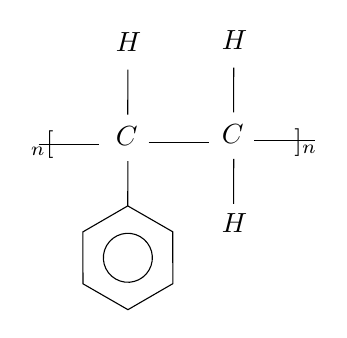
\begin{tikzpicture}[x=0.75pt,y=0.75pt,yscale=-1,xscale=1]
    	%uncomment if require: \path (0,992); %set diagram left start at 0, and has height of 992
    	
    	%Shape: Regular Polygon [id:dp6188045941784338] 
    	\draw  [fill={rgb, 255:red, 255; green, 255; blue, 255 }  ,fill opacity=1 ] (239.67,248.47) -- (218.04,261) -- (196.37,248.53) -- (196.33,223.53) -- (217.96,211) -- (239.63,223.47) -- cycle ;
    	%Straight Lines [id:da01235165655493664] 
    	\draw    (218,189.4) -- (217.96,211) ;
    	%Straight Lines [id:da9623385681374407] 
    	\draw    (218,145.4) -- (217.96,167) ;
    	%Straight Lines [id:da6542076497067413] 
    	\draw    (228,180.4) -- (257,180.4) ;
    	%Shape: Circle [id:dp4996181111574609] 
    	\draw  [fill={rgb, 255:red, 255; green, 255; blue, 255 }  ,fill opacity=1 ] (207.77,230.12) .. controls (211.02,224.47) and (218.23,222.52) .. (223.88,225.77) .. controls (229.53,229.02) and (231.48,236.23) .. (228.23,241.88) .. controls (224.98,247.53) and (217.77,249.48) .. (212.12,246.23) .. controls (206.47,242.98) and (204.52,235.77) .. (207.77,230.12) -- cycle ;
    	%Straight Lines [id:da806683426424035] 
    	\draw    (269,188.4) -- (268.96,210) ;
    	%Straight Lines [id:da13631583302127825] 
    	\draw    (269,144.4) -- (268.96,166) ;
    	%Straight Lines [id:da5408428644920109] 
    	\draw    (279,179.4) -- (308,179.4) ;
    	%Straight Lines [id:da16161616955769875] 
    	\draw    (175,181.4) -- (204,181.4) ;
    	
    	% Text Node
    	\draw (211,171.4) node [anchor=north west][inner sep=0.75pt]    {$C$};
    	% Text Node
    	\draw (211,126.4) node [anchor=north west][inner sep=0.75pt]    {$H$};
    	% Text Node
    	\draw (262,170.4) node [anchor=north west][inner sep=0.75pt]    {$C$};
    	% Text Node
    	\draw (262,125.4) node [anchor=north west][inner sep=0.75pt]    {$H$};
    	% Text Node
    	\draw (262,213.4) node [anchor=north west][inner sep=0.75pt]    {$H$};
    	% Text Node
    	\draw (297,172.4) node [anchor=north west][inner sep=0.75pt]    {$]_{n}$};
    	% Text Node
    	\draw (170,173.4) node [anchor=north west][inner sep=0.75pt]    {$_{n}[$};
    	
    	
    \end{tikzpicture}
    
    我们可以找到苯环的吸收峰.\\
    
    \begin{tabular}{|c|c|c|c|c|c|c|c|}
    	\hline
    	峰位置& 3026.01 & 1601.38 & 1583.11 & 1493.23 & 1452.51 & 755.35 & 695.79 \\
    	\hline
    	强度& 0.0988 & 9.749 & 40.546 & 0.178 & 0.191 & 1.078 & -0.0402 \\
    	\hline
    \end{tabular}\\
    
    我们也可以找到亚甲基的吸收峰.\\
    
    \begin{tabular}{|c|c|c|c|}
    	\hline
    	峰位置& 1452.51 & 2849.56 & 2922.45  \\
    	\hline
    	强度& 0.191 & 14.646 & 0.118  \\
    	\hline
    \end{tabular}
    \section{聚乙烯}
    
    
    \tikzset{every picture/.style={line width=0.75pt}} %set default line width to 0.75pt        
    
    \begin{tikzpicture}[x=0.75pt,y=0.75pt,yscale=-1,xscale=1]
    	%uncomment if require: \path (0,992); %set diagram left start at 0, and has height of 992
    	
    	%Straight Lines [id:da01235165655493664] 
    	\draw    (218,189.4) -- (217.96,211) ;
    	%Straight Lines [id:da9623385681374407] 
    	\draw    (218,145.4) -- (217.96,167) ;
    	%Straight Lines [id:da6542076497067413] 
    	\draw    (228,180.4) -- (257,180.4) ;
    	%Straight Lines [id:da806683426424035] 
    	\draw    (269,188.4) -- (268.96,210) ;
    	%Straight Lines [id:da13631583302127825] 
    	\draw    (269,144.4) -- (268.96,166) ;
    	%Straight Lines [id:da5408428644920109] 
    	\draw    (279,179.4) -- (308,179.4) ;
    	%Straight Lines [id:da16161616955769875] 
    	\draw    (175,181.4) -- (204,181.4) ;
    	
    	% Text Node
    	\draw (211,171.4) node [anchor=north west][inner sep=0.75pt]    {$C$};
    	% Text Node
    	\draw (211,126.4) node [anchor=north west][inner sep=0.75pt]    {$H$};
    	% Text Node
    	\draw (262,170.4) node [anchor=north west][inner sep=0.75pt]    {$C$};
    	% Text Node
    	\draw (262,125.4) node [anchor=north west][inner sep=0.75pt]    {$H$};
    	% Text Node
    	\draw (262,213.4) node [anchor=north west][inner sep=0.75pt]    {$H$};
    	% Text Node
    	\draw (298,172.4) node [anchor=north west][inner sep=0.75pt]    {$]_{n}$};
    	% Text Node
    	\draw (170,173.4) node [anchor=north west][inner sep=0.75pt]    {$_{n}[$};
    	% Text Node
    	\draw (209,214.4) node [anchor=north west][inner sep=0.75pt]    {$H$};
    	
    	
    \end{tikzpicture}\\
    
    我们也可以找到亚甲基的吸收峰.\\
    
    \begin{tabular}{|c|c|c|c|}
    	\hline
    	峰位置& 1452.51 & 2849.56 & 2922.45  \\
    	\hline
    	强度& 0.191 & 14.646 & 0.118  \\
    	\hline
    \end{tabular}\\
    
    我们也可以找到代表聚乙烯的吸收峰.\\
    
    \begin{tabular}{|c|c|c|}
    	\hline
    	峰位置&  719.58&1472.98 \\
    	\hline
    	强度& 35.853&22.202 \\
    	\hline
    \end{tabular}
    \section{利用聚乙烯找到聚苯乙烯链吸收峰}
    聚乙烯链的吸收峰为$k = 719.58cm^{-1}$.
    \[L = \frac{1}{2}m_1x_1'^2+\frac{1}{2}m_2x_2'^2-\frac{1}{2}k(x_1-x_2)^2\]
    \[\frac{\partial L}{\partial x_1}-\frac{d}{dt}\frac{\partial L}{\partial x'_1}=0\rightarrow m_1x_1''=k(x_2-x_1) \]
    \[\frac{\partial L}{\partial x_2}-\frac{d}{dt}\frac{\partial L}{\partial x'_2}=0\rightarrow m_1x_2''=-k(x_2-x_1) \]
    有\[x_1^{(4)}+\frac{k(m_1+m_2)}{m_1m_2}x_1^{(2)}=0\]
    
    \[\omega = \sqrt{\frac{k}{\mu}},\nu=\frac{1}{2\pi}\sqrt{\frac{k}{\mu}}\]
    
    我们可以得到$\nu\sim\mu^{-\frac{1}{2}}$,由于$k_\text{波数}=\frac{2\pi}{\lambda}=\frac{2\pi\nu}{v}$,则$k_\text{波数}\sim\mu^{-\frac{1}{2}}$.\\
    
    \[\mu_\text{聚苯乙烯} = \frac{m_1m_2}{m_1+m_2} = \frac{14\times90}{14+90} = 12.1153\]
    \[\mu_\text{聚乙烯} = \frac{m_1m_2}{m_1+m_2} = \frac{14\times14}{14+14} = 7\]
    则
    
    \[k_{\text{聚苯乙烯}} = \sqrt{\frac{\mu_{\text{聚乙烯}} }{\mu_{\text{聚苯乙烯}}}}k_{\text{聚乙烯}}=\sqrt{\frac{7}{12.1153}}\times719.58cm^{-1} = 546.96686cm^{-1}\]
    我们查阅表格和我们的测量值$538.55cm^{-1}$,很接近说明我们的近似大致正确(我们假设聚乙烯和聚苯乙烯的k相等)
    \section{对称性讨论}
    我们在文档已经使用对称性和群论讨论了振动类型和点群不等价不可约表示之间的关系,现在我们要讨论乙烯和苯环.
    \subsection{乙烯}
    
    
    \tikzset{every picture/.style={line width=0.75pt}} %set default line width to 0.75pt        
    
    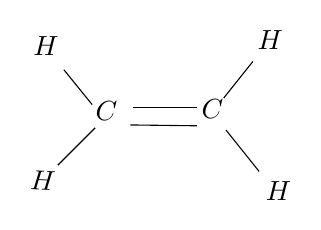
\begin{tikzpicture}[x=0.75pt,y=0.75pt,yscale=-1,xscale=1]
    	%uncomment if require: \path (0,992); %set diagram left start at 0, and has height of 992
    	
    	%Straight Lines [id:da01235165655493664] 
    	\draw    (212,185.4) -- (194,203.4) ;
    	%Straight Lines [id:da9623385681374407] 
    	\draw    (196.94,157.42) -- (210.55,174.19) ;
    	%Straight Lines [id:da806683426424035] 
    	\draw    (275,186.4) -- (291,206.4) ;
    	%Straight Lines [id:da13631583302127825] 
    	\draw    (288,153.4) -- (280.5,162.8) -- (273.96,171) ;
    	%Straight Lines [id:da24881701589378147] 
    	\draw    (230,175.4) -- (261,175.4) ;
    	%Straight Lines [id:da07016322307185907] 
    	\draw    (229,184) -- (261,184.4) ;
    	
    	% Text Node
    	\draw (211,171.4) node [anchor=north west][inner sep=0.75pt]    {$C$};
    	% Text Node
    	\draw (262,170.4) node [anchor=north west][inner sep=0.75pt]    {$C$};
    	% Text Node
    	\draw (289,137.4) node [anchor=north west][inner sep=0.75pt]    {$H$};
    	% Text Node
    	\draw (179.78,204.76) node [anchor=north west][inner sep=0.75pt]  [rotate=-2.83]  {$H$};
    	% Text Node
    	\draw (293,209.8) node [anchor=north west][inner sep=0.75pt]    {$H$};
    	% Text Node
    	\draw (181,140.4) node [anchor=north west][inner sep=0.75pt]    {$H$};
    	
    	
    \end{tikzpicture}
    
    分子对称群为$\textbf{D}_{2h}$,振动为:
    \[3A_{1g},1A_{1u},2B_{1g},1B_{1u},2B_{3u},1B_{2g},2B_{2u}\]
    \subsection{苯环}
    
    
    \tikzset{every picture/.style={line width=0.75pt}} %set default line width to 0.75pt        
    
    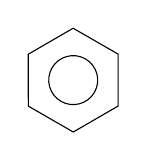
\begin{tikzpicture}[x=0.75pt,y=0.75pt,yscale=-1,xscale=1]
    	%uncomment if require: \path (0,992); %set diagram left start at 0, and has height of 992
    	
    	%Shape: Regular Polygon [id:dp6188045941784338] 
    	\draw  [fill={rgb, 255:red, 255; green, 255; blue, 255 }  ,fill opacity=1 ] (252.67,149.47) -- (231.04,162) -- (209.37,149.53) -- (209.33,124.53) -- (230.96,112) -- (252.63,124.47) -- cycle ;
    	%Shape: Circle [id:dp4996181111574609] 
    	\draw  [fill={rgb, 255:red, 255; green, 255; blue, 255 }  ,fill opacity=1 ] (220.77,131.12) .. controls (224.02,125.47) and (231.23,123.52) .. (236.88,126.77) .. controls (242.53,130.02) and (244.48,137.23) .. (241.23,142.88) .. controls (237.98,148.53) and (230.77,150.48) .. (225.12,147.23) .. controls (219.47,143.98) and (217.52,136.77) .. (220.77,131.12) -- cycle ;
    	
    	
    	
    	
    \end{tikzpicture}
    分子的对称群为$\textbf{D}_{6h}$群.其振动为\[2A_{1g},1A_{2g},1A_{2u},1B_{1g},1B_{1u},1B_{2g},3B_{2u},1E_{1g},3E_{1u},4E_{2g},2E_{2u}\]
    
\includepdf[pages=-, offset=0mm 0mm, scale=1.0]{aa.pdf}
    \newpage
    
\includepdf[pages=-, offset=0mm 0mm, scale=1.0]{1.pdf}
    
\end{document}